
\documentclass[ms.tex]{subfiles}
\begin{document}

\section{Discussion and Conclusions}
\label{sec:conclusions}

% fig 5
\begin{figure*}
\centering
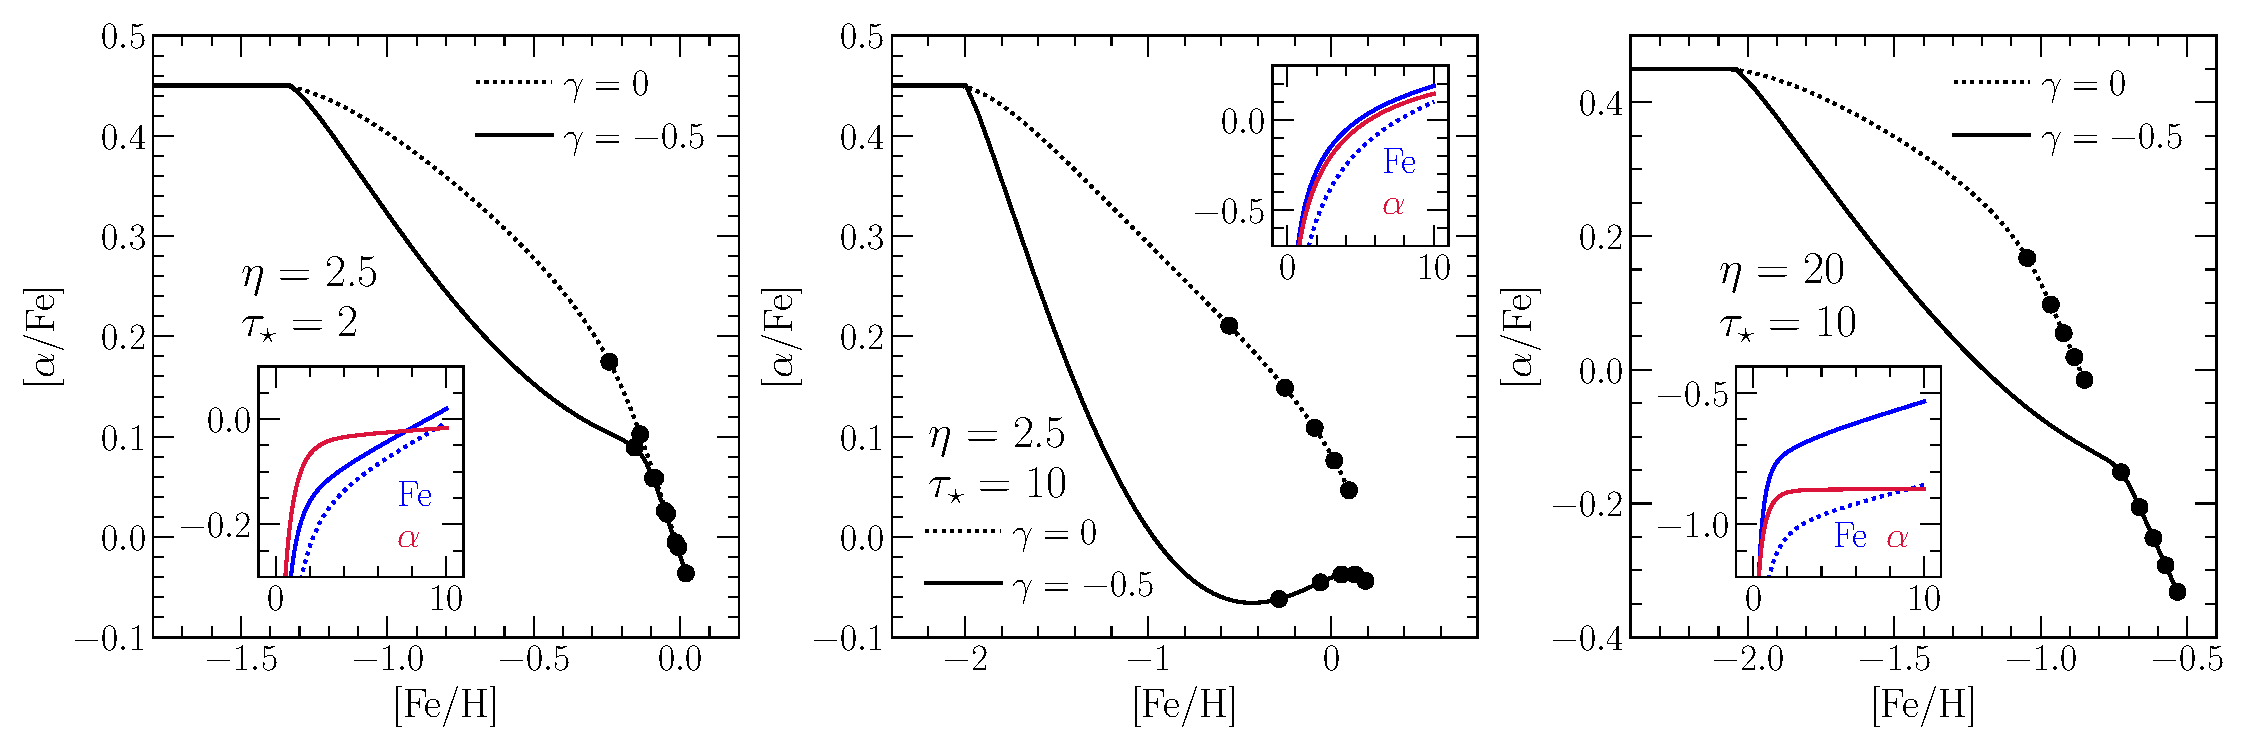
\includegraphics[scale = 0.47]{onezone_application.pdf}
\caption{
A comparison of one-zone galactic chemical evolution models based on
\citet[][for details, see their~\S~2]{Johnson2020} with ($\gamma = -0.5$,
solid) and without ($\gamma = 0$, dotted) metallicity-dependent SN Ia rates.
Tracks denote the O and Fe abundances in the interstellar medium parametrized
as a function of time with points marked at~$T = 2$, 4, 6, 8, and 10 Gyr.
Insets illustrate [O/H] and [Fe/H] as a function of time in Gyr for the
corresponding model.
We note on each panel the choice of the outflow mass-loading factor~$\eta$ and
the star formation efficiency timescale~$\tau_\star$.
}
\label{fig:onezone_app}
\end{figure*}

We have combined the mean SFHs of galaxies as predicted by the~\um~semi-analytic
model of galaxy formation~\citep{Behroozi2019} with the empirical MZR as
parametrized by~\citet{Zahid2014}.
Under the assumption that metallicity effects are the reason for the high
specific SN Ia rates observed in ASAS-SN~\citep{Brown2019} and
DES~\citep{Wiseman2021}, we have conducted simple numerical calculations to
investigate the origin of this effect.
Empirical constraints on the mass dependence of the specific SN Ia rate are
subject to uncertainties in the galaxy SMF at low stellar masses
(\citealp{Gandhi2022}; see also discussion of challenges in SMF measurements
in, e.g.,~\citealp{Weigel2016}).
Within our framework, however, we can theoretically predict the scaling of the
specific SN Ia rate with galaxy stellar mass in a manner that is independent of
the SMF (see equation~\ref{eq:specia}).
We find that the mean SFHs of galaxies of different stellar masses can account
for only a factor of~$\sim$2 increase in the specific SN Ia rate between
$10^{10}$ and~$10^{7.2}~\msun$.
If the rate scales with stellar mass as~$\dot{\text{N}}_\text{Ia} / \mstar \sim
\mstar^{-0.3}$, as suggested by the ASAS-SN~\citep{Brown2019} and DES
\citep{Wiseman2021} measurements normalized with the~\citet{Baldry2012} SMF,
then this is only~$\sim$30\% of the observed increase and an additional
metallicity dependence of~$Z^\gamma$ with~$\gamma \approx -0.5$ is required.
If instead the steeper scaling of~$\dot{\text{N}}_\text{Ia} / \mstar \sim
\mstar^{-0.5}$ derived by~\citet{Brown2019} is accurate, then stronger
scalings ($\gamma \approx -1.5$) are required, but~\citet{Gandhi2022}
demonstrate that scalings stronger than~$\gamma \lesssim -1$ fail to reproduce
the well-known correlations of [Mg/Fe] and [Fe/H] abundances as observed in M31
satellites by~\citet*{Vargas2014}.
\par
The realization that SN Ia rates could depend on metallicity with a
$\gamma = -0.5$ dependence has important implications for galactic chemical
evolution models.
To demonstrate this, we briefly explore a handful of one-zone models based
on~\citet{Johnson2020} which predict the evolution of O (produced only in
massive stars) and Fe (produced in both massive stars and SNe Ia); we refer
to their~\S~2 for details and note the differences here.
We take an exponential SFH with an e-folding timescale of~$\tau_\text{sfh} = 6$
Gyr and our minimum delay of~$t_\text{D} = 100$ Myr before the onset of SNe Ia
from a given stellar population.
For metallicity-dependent rates, we simply apply a~$(Z / Z_\odot)^{-0.5}$
prefactor to their Fe yield of~$y_\text{Fe}^\text{Ia} = 0.0017$, which assumes
that the shape of the DTD does not vary with metallicity -- only the
normalization.
Otherwise, these models are the same as~\citet{Johnson2020}.
\par
The left-hand panel of Fig.~\ref{fig:onezone_app} illustrates a model where we
take the same star formation efficiency timescale
($\tau_\star \equiv M_\text{gas} / \dot{M}_\star = 2$ Gyr) and
mass-loading factor describing the efficiency of outflows
($\eta \equiv \dot{M}_\text{out} / \dot{M}_\star = 2.5$) as in their fiducial
model.
The~$\gamma = -0.5$ case diverges from~$\gamma = 0$ near the ``knee''
in the evolutionary track in the gas-phase, but the two are similar at
near-solar abundances.
In a case where star formation is less efficient (e.g., $\tau_\star = 10$ Gyr;
middle panel), the differences are more dramatic.
Due to higher~$\tau_\star$, the knee occurs at much lower [Fe/H]
\citep{Weinberg2017}, and due to the extra SN Ia events relative to
$\gamma = 0$, the interstellar medium reaches~$\sim$solar [O/Fe] at much lower
[Fe/H].
With a near-solar equilibrium abundance, this model produces a ``secondary
plateau'' in [O/Fe] because the Fe enrichment rate slows down due to the
metallicity-dependence of the yield such that it is produced in similar ratios
as O (see inset).
In the right-hand panel, we now additionally strengthen outflows to~$\eta = 20$,
which lowers the equilibrium abundance to [Fe/H]~$\approx -1$ for~$\gamma = 0$.
Similar to the case shown in the left-hand panel,~$\gamma = -0.5$ deviates from
$\gamma = 0$ at the knee in the evolutionary track, but later ends up along an
extension of the~$\gamma = 0$ track, ending at a higher [Fe/H] and lower [O/Fe]
than~$\gamma = 0$ due to the enhanced Fe yield.
\par
These models are intended to be illustrative rather than quantitative.
In general, the only regions of chemical space where~$\gamma = 0$ and
$\gamma = -0.5$ make similar predictions are at near-solar abundances and along
the high [O/Fe] plateau, which occurs before the onset of SN Ia enrichment.
A~$\gamma = -0.5$ scaling has the strongest impact for dwarf galaxies where
star formation is inefficient~\citep[e.g.][]{Hudson2015} and the abundances are
low.
In these models, the latter arises due to strong outflows with a high
mass-loading factor as a consequence of the shallow gravity well.
\par
A scaling of~$\gamma = -0.5$ is in excellent agreement with the dependence of
the close binary fraction measured in APOGEE~\citep{Moe2019}, which suggests
that if a scaling of~$\dot{\text{N}}_\text{Ia} / \mstar \sim \mstar^{-0.3}$ is
accurate, then the elevated SN Ia rates in dwarf galaxies can be explained by a
combination of their more extended SFHs and an increased binary fraction
compared to their higher mass counterparts due to differences in their metal
content.
While~\citet{Gandhi2022} motivate their investigation from this viewpoint, here
we take this argument one step further and postulate that this accounts for
the~\textit{entire} increase in the specific SN Ia rate because the binary
fraction can naturally account for a factor of~$\sim$3 increase over
the~$\sim$1.5 decades in metallicity spanned by~$\mstar = 10^{7.2} - 10^{10}
\msun$ galaxies.
This interpretation goes against the hypothesis raised by~\citet{Kistler2013},
suggesting that the increased mass of WDs at low metallicities is a subdominant
effect.
Nonetheless, massive WDs at low metallicity may be an important component in
the theoretical understanding of the specific SN Ia rate as a function of
stellar mass if the steeper~$\sim \mstar^{-0.5}$ scaling inferred
by~\citet{Brown2019} is accurate.
\par
At first glance, an inverse dependence of SN Ia rates on metallicity may seem
at odds with the recent realization by~\citet{Holoien2022} that dwarf galaxy
hosts of SNe Ia detected by ASAS-SN tend to be oxygen-rich relative to similar
mass galaxies.
However, SN hosts detected by any survey are likely not a representative sample
of the underlying galaxy population because, due to the steeply declining
nature of the DTD~\citep[e.g.,][]{Maoz2012a}, the intrinsically highest SN Ia
rates should be in systems which experienced a recent starburst ($\lesssim$1
Gyr ago).
Since oxygen is produced mostly by massive stars with short lifetimes
\citep*[e.g.,][]{Hurley2000, Johnson2019}, these galaxies should also have a
higher-than-average oxygen abundance~\citep[e.g.,][]{Johnson2020}.
In other words, observed SN Ia hosts may be slightly metal-rich on average, but
one may arrive at a different conclusion if it were feasible to measure rates
within individual galaxies.
\par
The calculations we have presented here are simplified in several regards.
First, we have assumed the characteristic SFH predicted by a semi-analytic
model of galaxy formation at all stellar masses.
This approximation is reasonable for computing expected mean trends, but in
principle, the underlying galaxy population should occupy a distribution of
SFHs.
\citet{Brown2019} do not find strong evidence that the specific SN Ia rate
depends on star formation activity at the time of observation, but we do not
investigate this here because predicted SFHs on a galaxy-by-galaxy basis are
known to be highly model-dependent~\citep[e.g.][]{Li2020, Hu2022}.
Second, we have assumed that all galaxies lie perfectly on the MZR, which
should also be sufficient for computing mean trends.
However, similar to their SFHs and largely as a consequence thereof, galaxies
should populate a distribution of metallicities at fixed stellar mass.
Third, our metallicity scaling of~$Z^\gamma$ where~$Z$ is taken from the
\citet{Zahid2014} MZR assumes that all SNe Ia in any galaxy arise from stellar
populations whose metallicities are exactly that of the interstellar
medium implied by the MZR.
This approximation is also reasonable because models of galactic chemical
evolution suggest that galaxies should rapidly approach an equilibrium
abundance in which the production of new metals is balanced by dilution due to
accretion of metal-poor gas and losses to star formation and outflows
\citep{Larson1972, Weinberg2017}.
Characterizing metal abundances as an equilibrium phenomenon would suggest that
the young stellar populations which dominate the SN Ia rate (see
Fig.~\ref{fig:sfh_mzr} and discussion in~\S~\ref{sec:galprops}) should be of
similar metallicities -- at least on average.
Although the close binary fraction is known to increase at low abundances
in APOGEE~\citep{Badenes2018, Moe2019},~\citet{Mazzola2020} find that the
binary fraction decreases for stars with high [$\alpha$/Fe] ratios at fixed
[Fe/H], suggesting that the detailed chemical composition may significantly
impact stellar multiplicity.
Furthermore, the abundances of metals in stars is a many-dimensional quantity,
even when grouping them based on their various nucleosynthetic sources
\citep{Ting2022}.
However, a theoretical understanding of the metallicity dependence of SN Ia
rates is a relatively new topic in the literature, and a first-order
understanding of how the rates scale with the absolute metal abundance in
statistically average galaxies must be attained before considering how it
should scale with the detailed chemical composition of the progenitor
populations.

\end{document}
